\documentclass{article}
\usepackage[utf8]{inputenc} %кодировка
\usepackage[T2A]{fontenc}
\usepackage[english,russian]{babel} %русификатор 
\usepackage{mathtools} %библиотека матеши
\usepackage[left=1cm,right=1cm,top=2cm,bottom=2cm,bindingoffset=0cm]{geometry} %изменение отступов на листе
\usepackage{amsmath}
\usepackage{graphicx} %библиотека для графики и картинок
\graphicspath{}
\DeclareGraphicsExtensions{.pdf,.png,.jpg}
\usepackage{subcaption}
\usepackage{pgfplots}
\usepackage{array}
\usepackage{pgfplots}
\usepackage{multirow}
\usepackage{float}
\usepackage{derivative}

\begin{document}
% НАЧАЛО ТИТУЛЬНОГО ЛИСТА
\begin{center}
    \Large
    Федеральное государственное автономное \\
    образовательное учреждение высшего образования \\ 
    «Научно-образовательная корпорация ИТМО»\\
    \vspace{0.5cm}
    \large
    Факультет программной инженерии и компьютерной техники \\
    Направление подготовки 09.03.04 Программная инженерия \\
    \vspace{1cm}
    \Large
    \textbf{Отчёт по лабораторной работе №7} \\
    По дисциплине «Математическая статистика» (четвёртый семестр)\\
    Построение оценки линейной регрессии\\
    \large
    \vspace{8cm}

    \begin{minipage}{.33\textwidth}
    \end{minipage}
    \hfill
    \begin{minipage}{.4\textwidth}
    
        \textbf{Студент}: \vspace{.1cm} \\
        \ Дениченко Александр\\
        \ Разинкин Александр\\
        \ Соколов Анатолий\\
        \textbf{Практик}:  \\
        \ Милованович Екатерина Воиславовна
    \end{minipage}
    \vfill
Санкт-Петербург\\ 2024 г.
\end{center}
\thispagestyle{empty}

% КОНЕЦ ТИТУЛЬНОГО ЛИСТА 
\newpage
\section*{Цель работы}
Цель работы:

На основании анализа двумерной выборки

1. Построить точечную оценку линейной функции регрессии по методу средних и методу наименьших квадратов.

2. Проверить статистическую гипотезу об адекватности выбранной модели эксперементальным данным.

3. Построить доверительные интервалы для коэффиценков функции регрессии и для всей функции.
\section*{Данные }
Таблица данных:

\begin{table}[H]
    \centering
    \begin{tabular}{|c|c|c|c|c|c|}
    \hline
    $x(i)$&  5&  10&  16& 21& 29\\
    \hline
    $y(i)$&  36.7&  36.1&  36.5& 35.9& 40.1\\
    \hline
    \end{tabular}
\end{table}

Объём выборки n = 5

Доверительная вероятность $\beta = 0.95$

\section*{Линейная модель}
Формула:
\[y = a_0 + a_1x\]
\textbf{Метод средних:}

Исходя из таблицы, составили уравнения и сложили первые 2 и последнии 3

1)
\[36.7 = \tilde{a_0} + 5 \tilde{a_1}\]
\[+\]
\[36.1 = \tilde{a_0} + 10 \tilde{a_1}\]
\[=\]
\[72.8 = 2\tilde{a_0} + 15\tilde{a_1}\]

2)
\[36.5 = \tilde{a_0} + 16 \tilde{a_1}\]
\[+\]
\[35.9 = \tilde{a_0} + 21 \tilde{a_1}\]
\[+\]
\[40.1 = \tilde{a_0} + 29 \tilde{a_1}\]
\[=\]
\[37.5 = \tilde{a_0} + 22 \tilde{a_1}\]

3)
\[\begin{cases}
    2\tilde{a_0} + 15\tilde{a_1} = 72.8 \\
     \tilde{a_0} + 22 \tilde{a_1} = 37.5 
\end{cases}\]
\[\begin{cases}
    \tilde{a_0} \approx 35.831\\
    \tilde{a_1} \approx 0.076
\end{cases}\]

Получена точечная оценка:
\[\tilde{y} = 35.831 + 0.076x\]

\begin{center}
    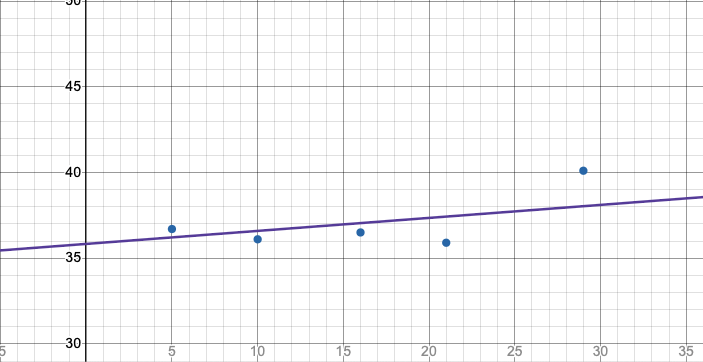
\includegraphics[width=.8\textwidth]{toch.png}\\
    График 1. Точечная оценка метод наименьших
\end{center}
\textbf{Метод наименьших квадратов:}
Для линейной функции
\[S(a_0,\ a_1) = \sum_{i=1}^{n}(y_i - \tilde{y}(x_i))^2 = \sum_{i=1}^{5}(y_i - \tilde{a_0} - \tilde{a_1}x_i)^2\ ->\ min\]
Найдём экстремум:
\[\begin{cases}
    \pdv{S}{a_0} = -2\left(\sum_{i=1}^{5}y_i - 5\tilde{a_0} - \tilde{a_1}\sum_{i=1}^{5}x_i\right) = 0\\
    \pdv{S}{a_1} = -2\left(\sum_{i=1}^{5}x_iy_i - \tilde{a_0}\sum_{i=1}^{5}x_i - \tilde{a_1}\sum_{i=1}^{5}x_i^2\right) = 0
\end{cases}\]
После подсчёта сумм получили систему:
\[\begin{cases}
    5\tilde{a_0} + 81\tilde{a_1} = 185.3\\
    81\tilde{a_0} + 1663\tilde{a_1} = 3045.3
\end{cases}\]
Подсчитали неизвестные:
\[\begin{cases}
    \tilde{a_0} = \frac{307423}{8770} \approx 35.054\\
    \tilde{a_1} = \frac{543}{4385} \approx0.124
\end{cases}\]
Подставили коэффиценты и получили точечную оценку:
\[\tilde{y} = 35.054+0.124x\]
\[S_{min}^{(1)} = \left(36.7-\frac{307423}{8770}\ -\ \frac{543}{4385}\cdot5\right)^{2}+\left(36.1-\frac{307423}{8770}\ -\ \frac{543}{4385}\cdot10\right)^{2}+\left(36.5-\frac{307423}{8770}\ -\ \frac{543}{4385}\cdot16\right)^{2}
+\]
\[+\left(35.9-\frac{307423}{8770}\ -\ \frac{543}{4385}\cdot21\right)^{2}+\left(40.1-\frac{307423}{8770}\ -\ \frac{543}{4385}\cdot29\right)^{2} \approx 6.573\]
\begin{center}
    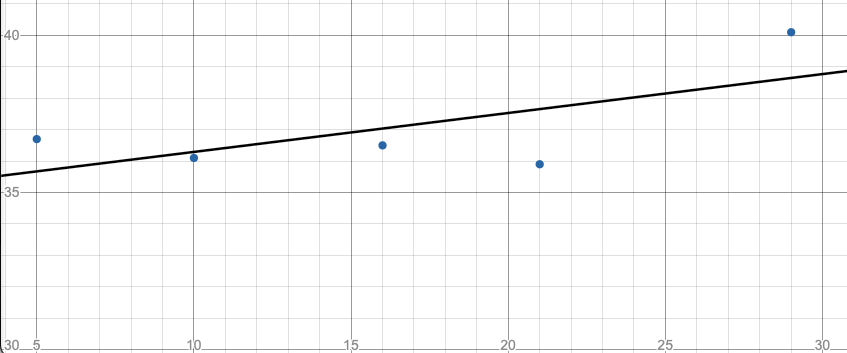
\includegraphics[width=.8\textwidth]{next.png}\\
    График 2. Точечная оценка МНК
\end{center}
\section*{Квадратичная модель}
Формула:
\[y = a_0 +a_1x+a_2x^2\]
\textbf{Метод наименьших квадратов:}
\[S(a_0, a_1, a_2) = \sum_{i=1}^{n}(y_i - \tilde{y}(x_i))^2 = \sum_{i=1}^{5}(y_i - \tilde{a_0} - \tilde{a_1}x_i - \tilde{a_2}x_i^2)^2 \ ->\ min\]


\[\begin{cases}
    \pdv{S}{a_0} = -2\left(\sum_{i=1}^{5}y_i - 5\tilde{a_0} - \tilde{a_1}\sum_{i=1}^{5}x_i - \tilde{a_2}\sum_{i=1}^{5}x_i^2\right) = 0\\
    \pdv{S}{a_1} = -2\left(\sum_{i=1}^{5}x_iy_i - \tilde{a_0}\sum_{i=1}^{5}x_i - \tilde{a_1}\sum_{i=1}^{5}x_i^2 - \tilde{a_2}\sum_{i=1}^{5}x_i^3\right) = 0\\
    \pdv{S}{a_2} = -2\left(\sum_{i=1}^{5}x_i^2y_i - \tilde{a_0}\sum_{i=1}^{5}x_i^2 - \tilde{a_1}\sum_{i=1}^{5}x_i^3 - \tilde{a_2}\sum_{i=1}^{5}x_i^4\right) = 0\\
\end{cases}\]
\[\sum_{i=1}^{5}y_i = 185.3\]
\[\sum_{i=1}^{5}x_i = 81\]
\[\sum_{i=1}^{5}x_i^2 = 1663\]
\[\sum_{i=1}^{5}x_i^3 = 38871\]
\[\sum_{i=1}^{5}x_i^4 = 977923\]
\[\sum_{i=1}^{5}x_iy_i = 3045.3\]
\[\sum_{i=1}^{5}x_i^2y_i = 63427.5\]

\[\begin{cases}
     5\tilde{a_0}+81\tilde{a_1}+1663\tilde{a_2} = 185.3\\
     81\tilde{a_0}+1663\tilde{a_1}+3887\tilde{a_2} = 3045.3\\
     1663\tilde{a_0}+38871\tilde{a_1}+977923\tilde{a_2} = 63427.5\\
\end{cases}\]

\[\begin{cases}
    \tilde{a_0} = \frac{2181415290553}{62080463050} = 35.139\\
    \tilde{a_1} = \frac{6839832}{1241609261} =0.006\\
    \tilde{a_2} = \frac{151658866}{31040231525} = 0.005\\
\end{cases}\]
Получена точечная оценка:
\[\tilde{y} = 35.139+0.006x+0.005x^2\]
\[S_{min}^{(2)} = \left(36.7-\frac{2181415290553}{62080463050}\ -\ \frac{6839832}{1241609261}\cdot5-\frac{151658866}{31040231525}\cdot5^{2}\right)^{2}+\]
\[+\left(36.1-\frac{2181415290553}{62080463050}\ -\ \frac{6839832}{1241609261}\cdot10-\frac{151658866}{31040231525}\cdot10^{2}\right)^{2}+\]
\[+\left(36.5-\frac{2181415290553}{62080463050}\ -\ \frac{6839832}{1241609261}\cdot16-\frac{151658866}{31040231525}\cdot16^{2}\right)^{2}+\]
\[+\left(35.9-\frac{2181415290553}{62080463050}\ -\ \frac{6839832}{1241609261}\cdot21-\frac{151658866}{31040231525}\cdot21^{2}\right)^{2}+\]
\[+\left(40.1-\frac{2181415290553}{62080463050}\ -\ \frac{6839832}{1241609261}\cdot29-\frac{151658866}{31040231525}\cdot29^{2}\right)^{2} = 4.925\]
\\
\begin{center}
    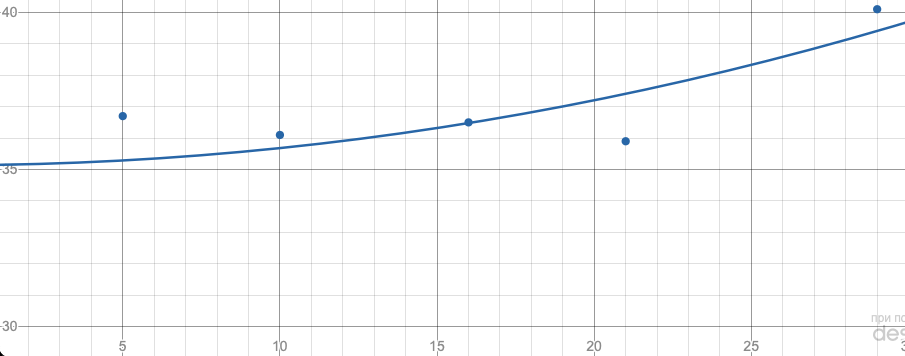
\includegraphics[width=.8\textwidth]{kvas.png}\\
    График 3. Точечная оценка МНК квадратичная регрессия
\end{center}
Сравнение графиков:
\begin{center}
    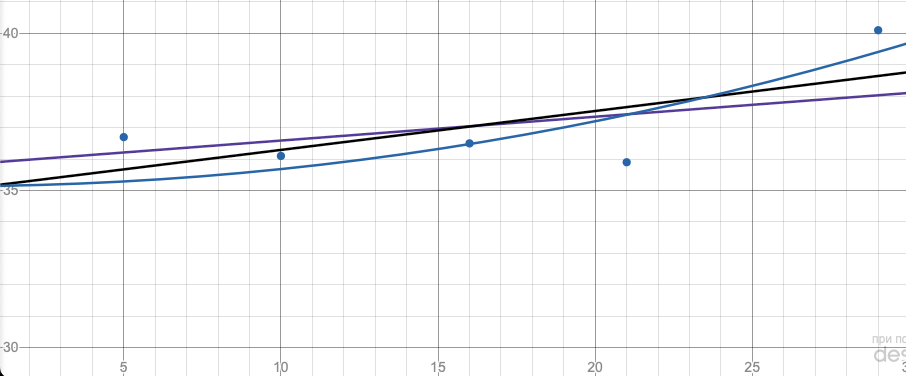
\includegraphics[width=.8\textwidth]{kvakva.png}\\
    График 4. Сравнение МНК квадратичная регрессия(синий), МНК линейная регрессия(чёрный), МС линейная регрессия(фиолетовый)
\end{center}

\section*{Гипотеза}
Проверка гипотезы об адекватности модели в задаче регрессии:

$H_0:$ Линейная модель хорошо согласуется с данными эксперемента и можно для дальнейшего исследования оставить её. Переход к квадратичной не требуется.

$H_1:$ Линейная модель плохо согласуется с данными эксперемента и можно для дальнейшего исследования оставить её. Переход к квадратичной требуется.
\\ \\
Введём статистический критерий Фишера:
\[F = \frac{\frac{1}{k-m}(S^{(1)}_{min} - S^{(2)}_{min})}{\frac{1}{n-k-1}S^{(2)}_{min}}\]

\[k=2;\ m=1;\ n=5\]
(n - количество эксперементальных данных)
\\
По теореме Фишера с уровнем значимости $\alpha = 0.05$ и степенями свободы $r_1 = k-m = 1$ и $r_2 = n-k-1 = 2$.
По таблице найдём:
\[F_{kr} = 18.51\]
\[F = \frac{\frac{1}{1}(6.573 - 4.925)}{\frac{1}{2}\cdot 4.925} \approx 0.669\]
Получили что F входит в допустимую область:
\[O = (0, F_{kr}) = (0, 18.51)\]
Тогда $H_0$ принимается и мы оставляем линейную модель.

\section*{Интервальные оценки параметров и функции регрессии}

\[y_i = a_0+a_1x_i+\varepsilon_i\]
$\varepsilon_i - $ ошибка измерения. Будем считать измерения равноточными.
\[\varepsilon_i \in N(0, D(\varepsilon_i) = \sigma^2)\]
\[\sigma^2 = \frac{S_{min}}{n-2} = \frac{6.573}{5-2} = 2.191\]
Определим оценку метрицы корреляционных моментов:

\[\tilde{K} = 
\begin{pmatrix}
    \tilde{\sigma}^2[\tilde{a_0}]& \tilde{K}[\tilde{a}_0, \tilde{a}_1]\\
    \tilde{K}[\tilde{a}_0, \tilde{a}_1] & \tilde{\sigma}^2[\tilde{a_1}]
\end{pmatrix}
= \tilde{\sigma}^2P^{-1}\]

\[P = 
\begin{pmatrix}
    5& \sum_{i=1}^{5}x_i\\
    \sum_{i=1}^{5}x_i& \sum_{i=1}^{5}x_i^2
\end{pmatrix}
=
\begin{pmatrix}
    5& 81\\
    81& 1663
\end{pmatrix}\]

\[P^{-1} = 
\frac{1}{detP}\cdot
\begin{pmatrix}
    1663& -81\\
    -81& 5
\end{pmatrix}=
\frac{1}{5\cdot 1663 - 81^2}
\begin{pmatrix}
    1663& -81\\
    -81& 5
\end{pmatrix}=
\frac{1}{1754}
\begin{pmatrix}
    1663& -81\\
    -81& 5
\end{pmatrix}
\]
Получили:
\[\tilde{\sigma}^2[\tilde{a_0}] =\frac{2.191}{1754}\cdot 1663 \approx 2.077\]
\[\tilde{\sigma}^2[\tilde{a_1}] =\frac{2.191}{1754}\cdot 5 \approx 0.006\]
\[\tilde{K}^2[\tilde{a_0}, \tilde{a_1}] =\frac{2.191}{1754}\cdot (-81) \approx -0.101\]
Оценка параметров:

По теореме Стьюдента с доверительной вероятностью $\beta = 0.9$ и степенью свободы $r = 3$ нашли по таблице:
\[t_{0.9; 3} = 1.638\]
Получили следующие оценки:

Для параметра $a_0$:
\[35.054 - 1.638\sqrt{2.077} < a_0 < 35.054 + 1.638\sqrt{2.077}\]
\[32.693 < a_0 < 37.415\]

Для параметра $a_1$:
\[0.124 - 1.638\sqrt{0.006} < a_1 < 0.124 + 1.638\sqrt{0.006}\]
\[-0.003 < a_1 < 0.251\]
\\
\\
Оценим функцию
\[\tilde{\sigma}^2[\tilde{y}(x)] = \tilde{\sigma}^2[\tilde{a_0}] + 2\tilde{K}[\tilde{a_0}, \tilde{a_1}]x + \tilde{\sigma}^2[\tilde{a_1}]x^2 = 2.077 - 0.202x+0.006x^2\]
\\ \\
Доверительный интервал на функцию регрессии:
\[35.054 + 0.124x - 1.638\sqrt{2.077 - 0.202x + 0.006x^2} < M[y/x] < 35.054 + 0.124x + 1.638\sqrt{2.077 - 0.202x + 0.006x^2}\]
\\ 
Для $x_1 = 5$:
\[35.054 + 0.124\cdot 5 - 1.638\sqrt{2.077 - 0.202\cdot 5 + 0.006\cdot (5)^2} < M[y/x_1] < 35.054 + 0.124\cdot 5 + 1.638\sqrt{2.077 - 0.202\cdot 5 + 0.006\cdot (5)^2}\]
\[33.867< M[y/x] <37.481\]
Для $x_2 = 10$:
\[35.054 + 0.124\cdot 10 - 1.638\sqrt{2.077 - 0.202\cdot 10 + 0.006\cdot (10)^2} < M[y/x_2] < 35.054 + 0.124\cdot 10 + 1.638\sqrt{2.077 - 0.202\cdot 10 + 0.006\cdot (10)^2}\]
\[34.966 < M[y/x_2] < 37.622\]
Для $x_3 = 16$:
\[35.054 + 0.124\cdot 16 - 1.638\sqrt{2.077 - 0.202\cdot 16 + 0.006\cdot (16)^2} < M[y/x_3] < 35.054 + 0.124\cdot 16 + 1.638\sqrt{2.077 - 0.202\cdot 16 + 0.006\cdot (16)^2}\]
\[36.027 < M[y/x_3] < 38.049\]
Для $x_4 = 21$:
\[35.054 + 0.124\cdot 21 - 1.638\sqrt{2.077 - 0.202\cdot 21 + 0.006\cdot (21)^2} < M[y/x_4] < 35.054 + 0.124\cdot 21 + 1.638\sqrt{2.077 - 0.202\cdot 21 + 0.006\cdot (21)^2}\]
\[ 36.522< M[y/x_4] < 38.794\]
Для $x_5 = 29$:
\[35.054 + 0.124\cdot 29 - 1.638\sqrt{2.077 - 0.202\cdot 29 + 0.006\cdot (29)^2} < M[y/x_5] < 35.054 + 0.124\cdot 29 + 1.638\sqrt{2.077 - 0.202\cdot 29 + 0.006\cdot (29)^2}\]
\[36.808< M[y/x_5] <40.492\]

\section*{Итоговый график}

\begin{center}
    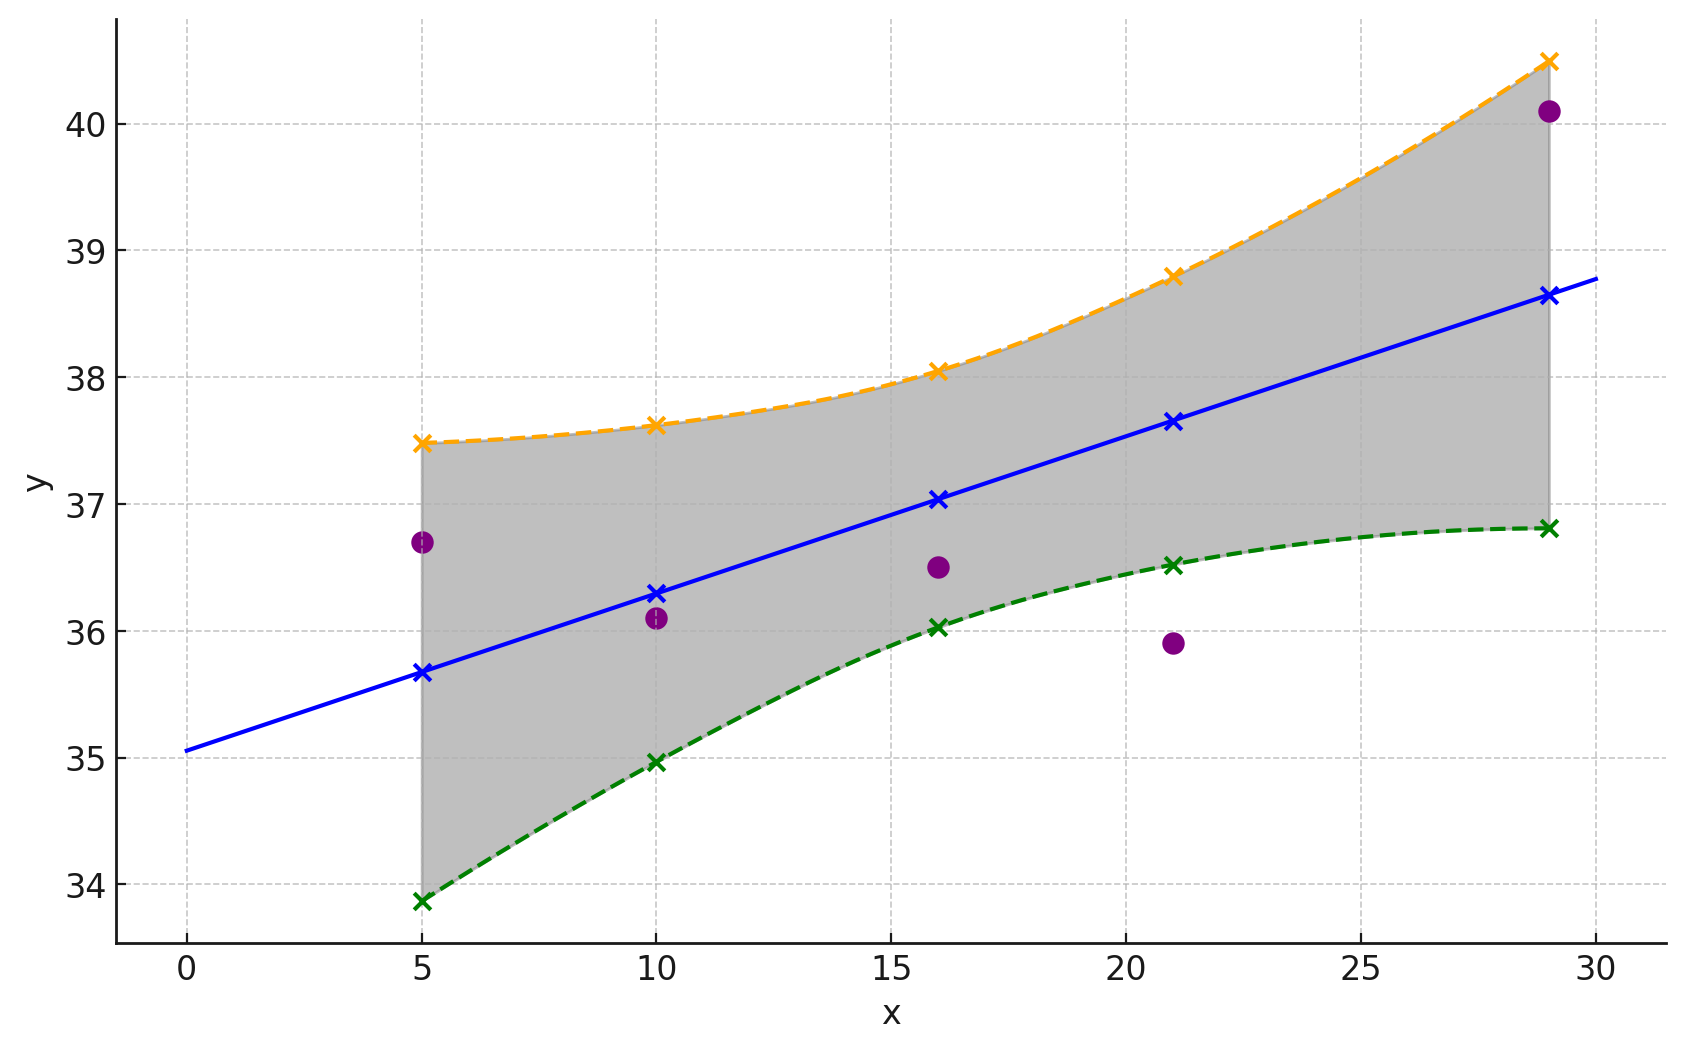
\includegraphics[width=.9\textwidth]{res.png}\\
    График 5. Доверительная область
\end{center}

\section*{Вывод}

На основании анализа двумерной выборки построили точечную оценку линейной функции регрессии по методу средних и методу наименьших квадратов.
Проверили статистическую гипотезу об адекватности выбранной модели эксперементальным данным.
Построили доверительные интервалы для коэффиценков функции регрессии и для всей функции.





\end{document}


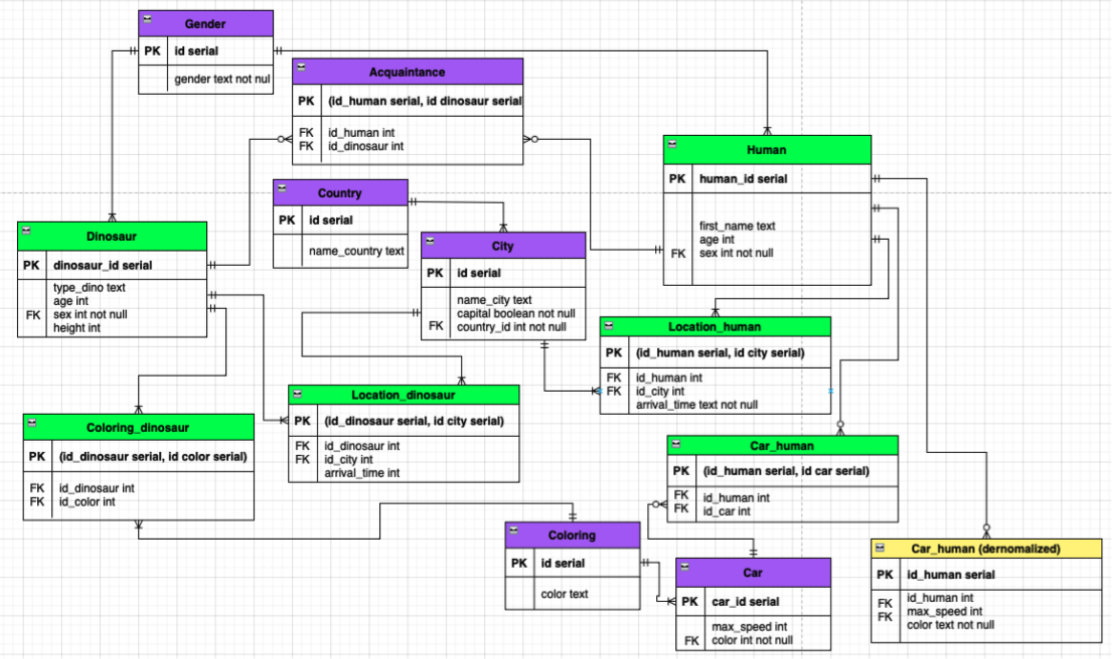
\includegraphics[width=.9\textwidth]{123}


